\section{Web-app amministratori}
\subsection{Introduzione}
La web app costituisce l'interfaccia tramite la quale l'amministratore può interagire col sistema.
Le funzionalità offerte sono:
\begin{itemize}
	\item login e logout;
	\item visualizzazione delle stanze e delle postazioni con i relativi stati;
	\item aggiunta, rimozione e modifica di stanze e postazioni;
	\item impostazione di postazioni come guaste;
	\item impostazione di stanze come inaccessibili;
	\item visualizzazione delle credenziali degli utenti;
	\item aggiunta, rimozione e modifica di credenziali;
	\item visualizzazione e scaricamento report sulle occupazioni e sulle igienizzazioni;
	\item visualizzazione di notifiche riguardanti il salvataggio dei dati sulla blockchain.
\end{itemize}

\subsection{Requisiti e installazione}
Il codice sorgente della web-app è pubblicato su GitHub all'indirizzo \url{https://github.com/DPCMGroup/bc19-webapp}.
Lo si può scaricare compresso in formato zip direttamente dal sito o, se si ha già installato il programma git, eseguendo il comando
\begin{verbatim}
	git clone https://github.com/DPCMGroup/bc19-webapp
\end{verbatim}

\subsubsection{Linguaggi}
\paragraph{Typescript}
Superset del linguaggio Javascript. Viene utilizzato per definire la logica dell'applicazione. \newline
Per poterlo utilizzare con Angular, esso va prima installato col comando \texttt{npm install -g typescript}

\paragraph{HTML}
Linguaggio di markup utilizzato per definire la struttura delle pagine web. Non necessita di installazione.

\paragraph{CSS}
Linguaggio per la definizione dello stile grafico delle pagine web. Nella nostra applicazione il codice css introdotto da noi è molto limitato perché, per questo, ci siamo affidati al framework Bootstrap. CSS non necessita di installazione.

\subsubsection{Tecnologie}
\paragraph{Node.js}
Programma focalizzato sull'esecuzione di codice javascript al di fuori del browser.
Per l'installazione fare riferimento alla pagina \url{https://nodejs.org/en/download/} 
\paragraph{npm}
Acronimo di Node Package Manager, permette di ottenere le librerie necessarie allo sviluppo.
Si ottiene insieme a Node.js tramite l'installazione di quest'ultimo.
\paragraph{Angular}
Framework per applicazioni web.
Per l'installazione fare riferimento alla pagina \url{https://angular.io/guide/setup-local#install-the-angular-cli}
\paragraph{Bootstrap}
Framework per la creazione di pagine web.
Per l'integrazione di Bootstrap in Angular fare riferimento alla pagina \url{https://www.npmjs.com/package/@ng-bootstrap/ng-bootstrap#installation}

\subsubsection{Test}
Per i test abbiamo utilizzato il framework Jasmine. Per utilizzarlo con Angular è necessario installarlo col comando \texttt{npm install -g jasmine} \newline
Per eseguire i test usare il comando \texttt{ng test} \newline
I test verranno eseguiti tramite il programma Karma e i loro risultati saranno visualizzati in una pagina del browser aperta automaticamente.

\subsubsection{IDE}
Per lo sviluppo abbiamo utilizzato l'IDE WebStorm. Per la sua installazione riferirsi alla pagina \url{https://www.jetbrains.com/webstorm/download/}

\subsubsection{Esecuzione}
Una volta installate le tecnologie sopra elencate si potrà eseguire la webapp aprendo un terminale nella root del progetto ed eseguendo il comando \texttt{ng serve} \newline
Verrà eseguito un server locale accessibile all'indirizzo \url{http://localhost:4200}

\subsection{Architettura}
L'architettura della web-app segue il modello a componenti imposto da Angular, che, a sua volta, si basa sul pattern Model-View-ViewModel, descritto dall'immagine sottostante.
\begin{figure}[H]
	\centering
	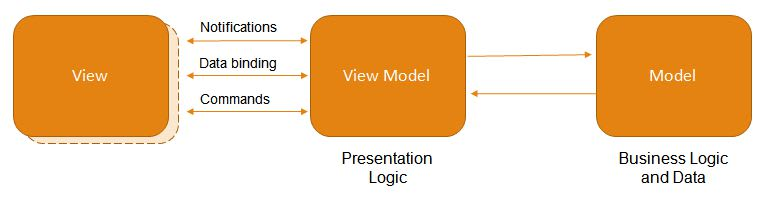
\includegraphics[width=15cm]{res/images/mvvm.jpg}
	\caption{Model-View-ViewModel}
	\label{fig:Model-View-ViewModel}
\end{figure}
Secondo questo modello la parte visiva del sito viene suddivisa in componenti, e ognuna di queste parti viene controllata da una diversa classe.
La parte visiva viene chiamata view, mentre la parte di controllo viene chiamata view model.
Un componente è costituito da 4 file. Nel seguente esempio è rappresentato un componente chiamato base.
\begin{verbatim}
	base.component.css
	base.component.html
	base.component.test.ts
	base.component.ts
\end{verbatim}
I file contengono, nell'ordine:
\begin{itemize}
	\item lo stile grafico del componente definito in css;
	\item la struttura del componente definito in html;
	\item i test definiti per il componente, scritti in typescript;
	\item il codice che definisce la logica del componente, scritto in typescript;
\end{itemize}

La struttura del sito è definita principalmente dal modo nel quale i componenti vengono annidati l'uno dentro all'altro. Nel codice html questo annidamento è descritto dai tag:
\begin{itemize}
	\item \texttt{<app-nomecomponente>}
	\item \texttt{<router-outlet>}
\end{itemize}
In entrambi i casi, nella pagina visualizzata, verrà inserito il componente specificato al posto del tag. Nel primo caso il componente da inserire è fisso ed è definito dal nome del tag stesso, nel secondo invece il componente inserito può variare. In quest'ultimo caso l'annidamento è definito dal'url col quale si sta visitando la pagina e dalla costante \texttt{routes} all'interno del file \texttt{src/app/app-routing.module.ts}.

\subsection{Diagrammi dei package}

\subsection{Diagrammi delle classi}
I diagrammi seguenti sono scritti secondo la sintassi UML. Le descrizioni testuali degli attributi e dei metodi delle classi riprendono alcune notazioni del linguaggio UML:
\begin{itemize}
	\item +/*/- prima del nome di un attributo o metodo indica che esso è, rispettivamente, pubblico, protetto o privato;
	\item i metodi e gli attributi il cui nome è sottolineato (\underline{nome\_esempio}) sono statici.
\end{itemize}
\subsubsection{Login}
\begin{figure}[H]
	\centering
	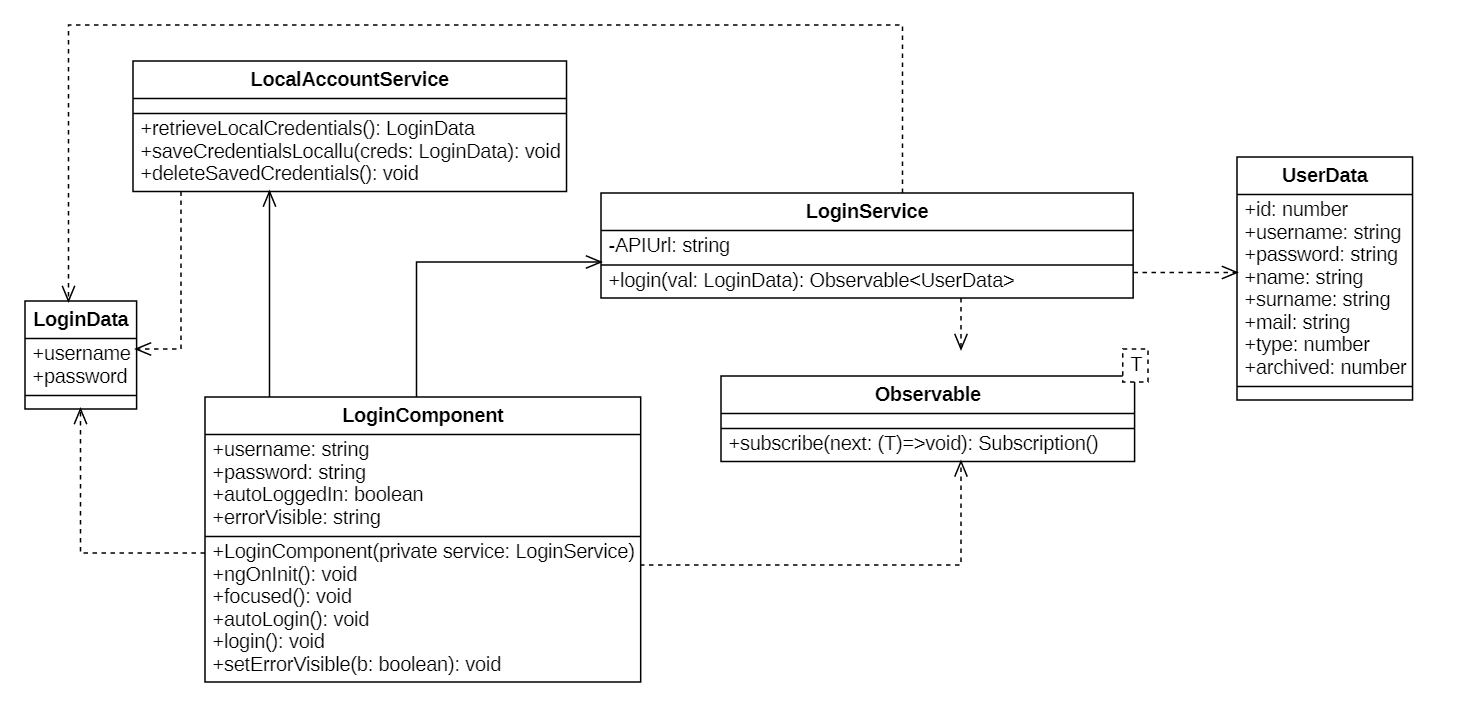
\includegraphics[width=18cm]{res/images/webapp-login-diagrammaClassi.png}
	\caption{Diagramma delle classi per il login}
	\label{fig:DiagrammaClassiLogin}
\end{figure}
Nel diagramma sovrastante sono rappresentate le classi utilizzate dalla pagina di login e le dipendenze tra di esse. La classe \texttt{LoginComponent} dirige la gestione del login manuale, tramite inserimento delle credenziali da parte dell'utente, e di quello automatico, tramite verifica delle credenziali precedentemente salvate nel local storage del browser. A \texttt{LoginService}, in particolare, viene delegata la verifica delle credenziali tramite il server, mentre a LocalAccountService, vengono delegate la scrittura, la lettura e l'eliminazione delle credenziali salvate nel browser. Per comunicare credenziali di accesso da una classe all'altra, viene utilizzata \texttt{LoginData}. \texttt{UserData} invece viene usata per la ricezione dal server dei dati dell'utente che si è autenticato.

\paragraph{Classi}

\subparagraph{LoginComponent}
Classe che si occupa della gestione del login manuale, ovvero tramite l'inserimento delle credenziali da parte dell'utente, e di quello automatico, ovvero tramite l'utilizzo delle credenziali precedentemente salvate nel local storage del browser. \newline
\textbf{Attributi}
\begin{itemize}
	\item \texttt{+ username: string}
	\item \texttt{+ password: string}
	\item \texttt{+ autoLoggedIn: boolean}
	\item \texttt{+ errorVisible: string}
\end{itemize}
\textbf{Metodi}
\begin{itemize}
	\item \texttt{+ constructor(private loginService: LoginService, private localAccountService: LocalAccountService)}
	\item \texttt{+ ngOnInit(): void} \newline
	Metodo che viene chiamato all'inizializzazione delle pagina. Provoca l'evento di login automatico.
	\item \texttt{+ focused(): void} \newline
	Metodo che viene chiamato nel momento in cui uno dei due campi di inserimento delle credenziali viene selezionata. Provoca l'impostazione dell'invisibilità dell'errore che indica l'incorrettezza delle credenziali inserite.
	\item \texttt{+ autoLogin(): void} \newline
	Metodo che effettua un tentativo di autenticazione con le credenziali salvate nel local storage. Se l'autenticazione riesce l'utente viene reindirizzato alla pagina home. Altrimenti viene visualizzata la pagina di inserimento delle credenziali.
	\item \texttt{+ login(): void} \newline
	Metodo che effettua un tentativo di autenticazione con le credenziali inserite dall'utente. Se l'autenticazione riesce l'utente viene reindirizzato alla pagina home. Altrimenti viene mostrato un messaggio di errore.
	\item \texttt{+ setErrorVisible(b: boolean): void} \newline
	Metodo che imposta la visibilità dell'errore che indica l'incorrettezza delle credenziali inserite.
\end{itemize}
\subparagraph{LoginService}
Servizio che permette di verificare tramite il server la validità di credenziali per l'autenticazione. Ogni metodo di questa classe, tranne il costruttore, restituisce un \texttt{Observable}. Questo oggetto espone un metodo subscribe con il quale si potrà impostare una funzione di callback che verrà chiamata quando il server fornirà una risposta. \newline
\textbf{Attributi}
\begin{itemize}
	\item \texttt{- APIUrl: string}
	L'url base dell'API REST a cui il servizio fa riferimento.
\end{itemize}
\textbf{Metodi}
\begin{itemize}
	\item \texttt{+ login(val: LoginData): Observable<UserData>} \newline
	Verifica l'esistenza delle credenziali passate come parametro nel database. Restituisce un Observable che permette di ottenere, in un \texttt{UserData}, i dati dell'utente corrispondente alle credenziali.
\end{itemize}
\subparagraph{LocalAccountService}
Servizio che permette di gestire il salvataggio delle credenziali dell'utente nel local storage del browser. \newline
\textbf{Metodi}
\begin{itemize}
	\item \texttt{+ retrieveLocalCredentials(): LoginData}
	\item \texttt{+ saveCredentialsLocally(creds: LoginData): void}
	\item \texttt{+ deleteSavedCredentials(): void}
\end{itemize}
\subparagraph{LoginData}
Classe che contiene i valori necessari per l'autenticazione di un amministratore al sistema. Viene usata per la comunicazione di questo tipo di dati all'interno dell'applicazione. \newline
\textbf{Attributi}
\begin{itemize}
	\item \texttt{+ username: string}
	\item \texttt{+ password: string}
\end{itemize}
\subparagraph{UserData}
Classe che contiene tutti e soli i valori necessari per il salvataggio di un utente sul database. È utilizzata per il transito dei dati degli utenti all'interno dell'applicazione. \newline
\textbf{Attributi}
\begin{itemize}
	\item \texttt{+ id: number}
	\item \texttt{+ username: string}
	\item \texttt{+ password: string}
	\item \texttt{+ name: string}
	\item \texttt{+ surname: string}
	\item \texttt{+ mail: string}
	\item \texttt{+ type: number}
	\item \texttt{+ archived: number}
\end{itemize}
\subparagraph{Observable<T>}
Classe fornita dalla libreria Rxjs. Viene utilizzata per effettuare chiamate asincrone al server. Per una documentazione più approfondita fare riferimento a \url{https://angular.io/guide/rx-library}. \newline
\textbf{Metodi}
\begin{itemize}
	\item \texttt{+ subscribe(next: (T)=>void): Subscription} \newline
	Metodo che permette di eseguire la chiamata al server e di specificare la funzione di callback che gestirà la risposta.
\end{itemize}

\subsubsection{Gestione stanze e postazioni}
\begin{figure}[H]
	\centering
	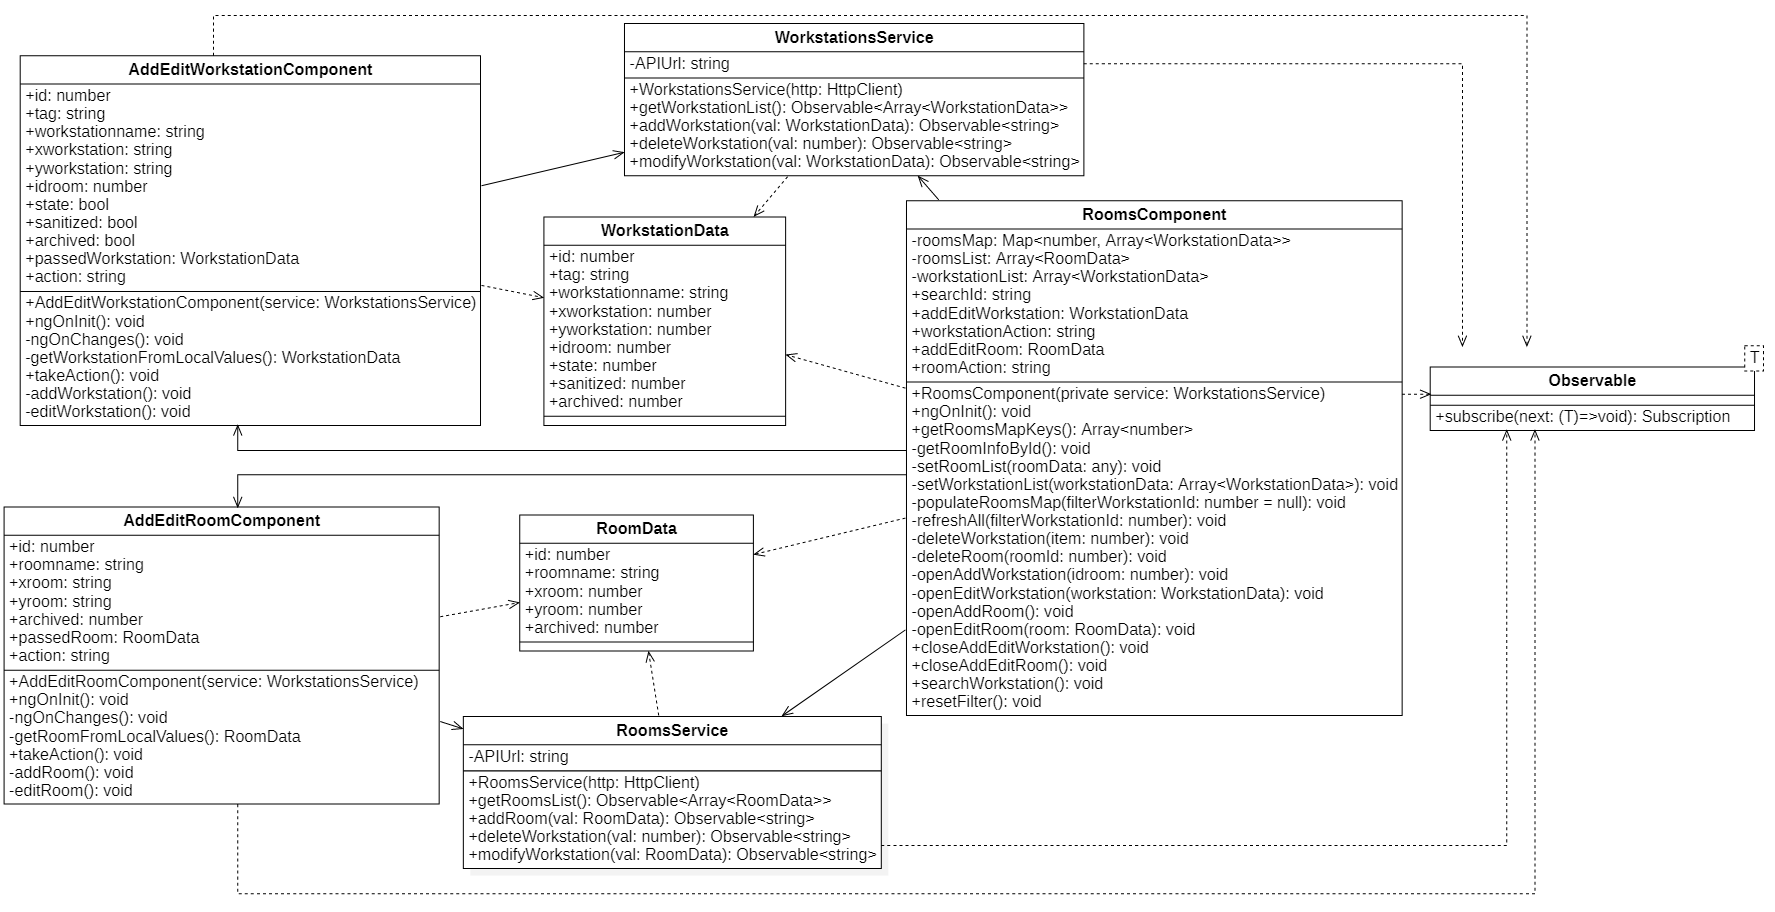
\includegraphics[width=18cm]{res/images/webapp-visualAddEditStanzePostazioni-diagrammaClassi.png}
	\caption{Diagramma delle classi per la gestione delle stanze e delle postazioni}
	\label{fig:DiagrammaClassiStanzePostazioni}
\end{figure}
Il diagramma sovrastante rappresenta l'architettura utilizzata per la pagina di gestione delle stanze e delle postazioni. \newline
\texttt{RoomsComponent} si occupa della visualizzazione ed eliminazione delle stanze e delle postazioni. Essa delega la creazione e modifica dei questi due dati alle classi \texttt{AddEditWorkstationComponent} e \texttt{AddEditRoomComponent}. Le tre componenti contengono un riferimento ad ognuno dei servizi di cui necessitano. I due servizi coinvolti sono \texttt{WorkstationService} e \texttt{RoomService}. Le informazini vengono ottenute dal server tramite la classe \texttt{Observable}. In generale i dati riguardanti postazioni e stanze sono scambiati utilizzando le due classi \texttt{WorkstationData} e \texttt{RoomData}.


\paragraph{Classi}
\subparagraph{RoomsComponent}
Classe che si occupa della visualizzazione, eliminazione e, tramite i componenti AddEditWorkstation e AddEditRoom, dell'aggiunta e modifica di postazioni e stanze. \newline
\textbf{Attributi}
\begin{itemize}
	\item \texttt{- roomsMap: Map<number, Array<WorkstationData>>} \newline
		Map in cui ad ogni stanza sono assegnate le sue postazione, ovvero quelle con \texttt{idroom} uguale all'\texttt{id} della stanza. Se l'utente applica un filtro alla lista, qui verranno contenute solo le stanze e le postazioni selezionate da tale filtro.
	\item \texttt{- roomsList: Array<RoomsData>} \newline
		Array utilizzato per contenere le stanze ottenutedal server
	\item \texttt{- workstationList: Array<Workstation>} \newline
		Array utilizzato per contenere le postazioni ottenute dal server.
	\item \texttt{+ searchId: string} \newline
		Id specificato dall'utente per la ricerca di una postazione.
	\item \texttt{+ addEditWorkstation: WorkstationData} \newline
		Contiene i dati della postazione che verrà aggiunta o modificata.
	\item \texttt{+ workstationAction: string} \newline
		Valore specificato dall'utente che provocherà la modifica o l'aggiunta della postazione salvata in \texttt{addEditWorkstation}
	\item \texttt{+ addEditRoom: RoomData} \newline
		Contiene i dati della stanza che verrà aggiunta o modificata.
	\item \texttt{+ roomAction: string} \newline
		Valore specificato dall'utente che provocherà la modifica o l'aggiunta della stanza salvata in \texttt{addEditRoom}
\end{itemize}
\textbf{Metodi}
\begin{itemize}
	\item \texttt{+ constructor(private service: SharedService, private cd: ChangeDetectorRef)} 
	\item \texttt{+ ngOnInit(): void} \newline
	Questa funzione viene chiamata all'inizializzazione della pagina.
	\item \texttt{+ getRoomsMapKeys(): Array<number>} \newline
	Restituisce un array con gli id delle stanze contenute in \texttt{roomsMap}
	\item \texttt{- getRoomInfoById(id: number): RoomData} \newline
	Restituisce un oggetto \texttt{RoomData} con i dati della stanza identificata dall'id passato come parametro.
	\item \texttt{- setRoomList(roomData: Array<RoomData>): void} \newline
	Reinizializza \texttt{roomList} con i dati ricevuti
	\item \texttt{- setWorkstationList(workstationData: Array<WorkstationData>): void} \newline
	Reinizializza \texttt{workstationList} con i dati ricevuti
	\item \texttt{- populateRoomsMap(filterWorkstationId: number): void} 
	Reinizializza \texttt{roomsMap} ponendo come chiavi gli id delle stanze contenute in \texttt{roomList} e come valori le postazioni contenute nelle rispettive stanze. \newline
	Se non viene specificato l'attributo \texttt{filterWorkstationId} nella mappa vengono inserite anche le stanze vuote. \newline
	Se viene specificato l'attributo \texttt{filterWorkstationId} verrà inserita nella mappa solo la postazione con l'id indicato e la stanza che la contiene.
	\item \texttt{- refreshAll(filterWorkstationId: number): void} \newline
	Richiede al server le stanze e le postazione e le organizza, tramite \texttt{populateRoomsMap}, in una mappa. Il parametro \texttt{filterWorkstationId} viene passato direttamente a \texttt{populateRoomsMap}
	\item \texttt{- deleteWorkstation(item: number): void} \newline
	Richiede al server l'eliminazione della postazione con l'id specificato
	\item \texttt{- deleteRoom(roomId: number): void} \newline
	Richiede al server l'eliminazione della stanza con l'id specificato
	\item \texttt{- openAddWorkstation(idroom: number): void} \newline
	Rende visibile il form per l'aggiunta di una postazione. Inoltre imposta i parametri necessari all'esecuzione di questa azione.
	\item \texttt{- openEditWorkstation(workstation: WorkstationData): void} \newline
	Rende visibile il form per la modifica di una postazione. Inoltre imposta i parametri necessari all'esecuzione di questa azione. 
	\item \texttt{- openAddRoom(): void} \newline
	Rende visibile il form per l'aggiunta di una stanza. Inoltre imposta i parametri necessari all'esecuzione di questa azione.
	\item \texttt{- openEditRoom(room: RoomData): void} \newline
	Rende visibile il form per la modifica di una stanza. Inoltre imposta i parametri necessari all'esecuzione di questa azione.
	\item \texttt{+ closeAddEditWorkstation(): void} \newline
	Provoca l'aggiornamento dei dati contenuti nella pagina.
	\item \texttt{+ closeAddEditRoom(): void} \newline
	Provoca l'aggiornamento dei dati contenuti nella pagina.
	\item \texttt{+ searchWorkstation(): void} \newline
	Richiede tutti i dati sulle postazioni e sulle stanze al server specificando il filtro indicato dall'utente.
	\item \texttt{+ resetFilter(): void} \newline
	Richiede tutti i dati sulle postazioni e sulle stanze al server senza alcun filtro.
\end{itemize}
	
\subparagraph{AddEditWorkstationComponent}
Classe che si occupa dell'aggiunta e modifica di postazioni. I primi 9 attributi sono sempre sincronizzati con il form che viene presentato all'utente. Tramite essi viene definita la postazione da aggiungere o i nuovi dati della postazione da modificare.\newline
\textbf{Attributi}
\begin{itemize}
	\item \texttt{+ id: number } 
	\item \texttt{+ tag: string } 
	\item \texttt{+ workstationname: string } 
	\item \texttt{+ xworkstation: string } 
	\item \texttt{+ yworkstation: string } 
	\item \texttt{+ idroom: number } 
	\item \texttt{+ state: bool } 
	\item \texttt{+ sanitized: bool } 
	\item \texttt{+ archived: bool } 
	\item \texttt{+ passedWorkstation: WorkstationData } \newline
	L'oggetto che viene passato da \texttt{RoomComponent} e che indica la postazione da modificare.
	\item \texttt{+ action: string} \newline
	L'attributo che viene passato da \texttt{RoomComponent} e che indica il tipo di azione da eseguire: aggiunta o modifica della postazione;
\end{itemize}
\textbf{Metodi}
\begin{itemize}
	\item \texttt{+ constructor(service: WorkstationsService) }
	\item \texttt{- ngOnChanges(): void } \newline
	Metodo chiamato ogni volta che una proprietà data-bound viene modificata. In questo caso serve per aggiornare i parametri locali in base ai valori di \texttt{passedWorkstation}.
	\item \texttt{- getWorkstationFromLocalValues(): WorkstationData } \newline
	Restituisce un oggetto \texttt{WorkstationData} ottenuto dai primi 9 attributi.
	\item \texttt{+ takeAction(): void } \newline
	Chiama il metodo \texttt{addWorkstation()} o \texttt{editWorkstation()} a seconda del valore dell'attributo action.
	\item \texttt{- addWorkstation(): void } \newline
	Richiede al service di aggiungere la postazione specificata.
	\item \texttt{- editWorkstation(): void} \newline
	Richiede al service di modificare la postazione nel modo specificato.
	
\end{itemize}
\subparagraph{AddEditRoomComponent}
Classe che si occupa dell'aggiunta e modifica di stanze. I primi 5 attributi sono sempre sincronizzati con il form che viene presentato all'utente. Tramite essi viene definita la stanza da aggiungere o i nuovi dati della stanza da modificare.\newline
\textbf{Attributi}
\begin{itemize}
	\item \texttt{+ id: number 	}
	\item \texttt{+ roomname: string 	}
	\item \texttt{+ xroom: string 	}
	\item \texttt{+ yroom: string 	}
	\item \texttt{+ archived: number 	}
	\item \texttt{+ noticeChangeVariable: boolean 	}
	\item \texttt{+ passedRoom: RoomData 	} \newline
	L'oggetto che viene passato da \texttt{RoomComponent} e che indica la stanza da modificare.
	\item \texttt{+ action: string} \newline
	L'attributo che viene passato da \texttt{RoomComponent} e che indica il tipo di azione da eseguire: aggiunta o modifica della stanza;
\end{itemize}
\textbf{Metodi}
\begin{itemize}
	\item \texttt{+ constructor(service: WorkstationsService) 	}
	\item \texttt{- ngOnChanges(): void 	} \newline
	Metodo chiamato ogni volta che una proprietà data-bound viene modificata. In questo caso serve per aggiornare i parametri locali in base ai valori di \texttt{passedRoom}.
	\item \texttt{- getRoomFromLocalValues(): RoomData 	} \newline
	Restituisce un oggetto \texttt{RoomData} ottenuto dai primi 5 attributi.
	\item \texttt{+ takeAction(): void 	} \newline
	Chiama il metodo \texttt{addRoom()} o \texttt{editRoom()} a seconda del valore dell'attributo action.
	\item \texttt{- addRoom(): void 	} \newline
	Richiede al service di aggiungere la stanza specificata.
	\item \texttt{- editRoom(): void} \newline
	Richiede al service di modificare la postazione nel modo specificato.
\end{itemize}
\subparagraph{WorkstationsService}
Servizio che permette di ottenere dal server informazioni sulle postazioni. Ogni metodo di questa classe, tranne il costruttore, restituisce un \texttt{Observable}. Questo oggetto espone un metodo subscribe con il quale si potrà impostare una funzione di callback che verrà chiamata quando il server fornirà una risposta. \newline
\textbf{Attributi}
\begin{itemize}
	\item \texttt{- APIUrl: string} \newline
	L'url base dell'API REST a cui il servizio fa riferimento.
\end{itemize}
\textbf{Metodi}
\begin{itemize}
	\item \texttt{+ constructor(http: HttpClient) 	}
	\item \texttt{+ getWorkstationList(): Observable<Array<WorkstationData>> 	} \newline
	Usato per ottenere una lista delle postazioni.
	\item \texttt{+ addWorkstation(val: WorkstationData): Observable<string> 	} \newline
	Usato per tentare di aggiungere la postazione indicata in \texttt{val} e di ricevere l'esito dell'operazione.
	\item \texttt{+ deleteWorkstation(val: number): Observable<string> 	} \newline
	Usato per tentare di eliminare la postazione con id \texttt{val} e di ricevere l'esito dell'operazione.
	\item \texttt{+ modifyWorkstation(val: WorkstationData): Observable<string>} \newline
	Usato per tentare di modificare la postazione con id pari a quello contenuto in \texttt{val} assegnandole gli altri valori dello stesso parametro. Restituisce, tramite un \texttt{Observable}, una risposta in formato stringa che indica l'esito dell'operazione.
\end{itemize}
\subparagraph{RoomsService}
Servizio che permette di ottenere dal server informazioni sulle stanze. Ogni metodo di questa classe, tranne il costruttore, restituisce un \texttt{Observable}. Questo oggetto espone un metodo subscribe con il quale si potrà impostare una funzione di callback che verrà chiamata quando il server fornirà una risposta. \newline
\textbf{Attributi}
\begin{itemize}
	\item \texttt{- APIUrl: string} \newline
	L'url base dell'API REST a cui il servizio fa riferimento.
\end{itemize}
\textbf{Metodi}
\begin{itemize}
	\item \texttt{+ constructor(http: HttpClient) 	}
	\item \texttt{+ getRoomsList(): Observable<Array<RoomData>> 	} \newline
	Usato per ottenere una lista delle stanze.
	\item \texttt{+ addRoom(val: RoomData): Observable<string> 	} \newline
	Usato per tentare di aggiungere la stanza indicata in \texttt{val} e di ricevere l'esito dell'operazione.
	\item \texttt{+ deleteWorkstation(val: number): Observable<string> 	} \newline
	Usato per tentare di eliminare la stanza con id \texttt{val} e di ricevere l'esito dell'operazione.
	\item \texttt{+ modifyWorkstation(val: RoomData): Observable<string>} \newline
	Usato per tentare di modificare la stanza con id pari a quello contenuto in \texttt{val} assegnandole gli altri valori dello stesso parametro. Restituisce, tramite un \texttt{Observable}, una risposta in formato stringa che indica l'esito dell'operazione.
\end{itemize}
\subparagraph{WorkstationData}
Classe che contiene tutti e soli i valori necessari per il salvataggio di una postazione sul database. È utilizzata per il transito dei dati delle postazioni all'interno dell'applicazione. \newline
\textbf{Attributi}
\begin{itemize}
	\item \texttt{+ id: number 	}
	\item \texttt{+ tag: string 	}
	\item \texttt{+ workstationname: string 	}
	\item \texttt{+ xworkstation: number 	}
	\item \texttt{+ yworkstation: number 	}
	\item \texttt{+ idroom: number 	}
	\item \texttt{+ state: number 	}
	\item \texttt{+ sanitized: number 	}
	\item \texttt{+ archived: number}
\end{itemize}
\subparagraph{RoomData}
Questa classe contiene tutti e soli i valori necessari per il salvataggio di una stanza sul database. È utilizzata per il transito dei dati delle stanze all'interno dell'applicazione. \newline
\textbf{Attributi}
\begin{itemize}
	\item \texttt{+ id: number 	}
	\item \texttt{+ roomname: string 	}
	\item \texttt{+ xroom: number 	}
	\item \texttt{+ yroom: number 	}
	\item \texttt{+ archived: number}
\end{itemize}
\subparagraph{Observable<T>}
Classe fornita dalla libreria Rxjs. Viene utilizzata per effettuare chiamate asincrone al server. Per una documentazione più approfondita fare riferimento a \url{https://angular.io/guide/rx-library}. \newline
\textbf{Metodi}
\begin{itemize}
	\item \texttt{+ subscribe(next: (T)=>void): Subscription} \newline
	Metodo che permette di eseguire la chiamata al server e di specificare la funzione di callback che gestirà la risposta.
\end{itemize}

\subsubsection{Gestione credenziali}
\begin{figure}[H]
	\centering
	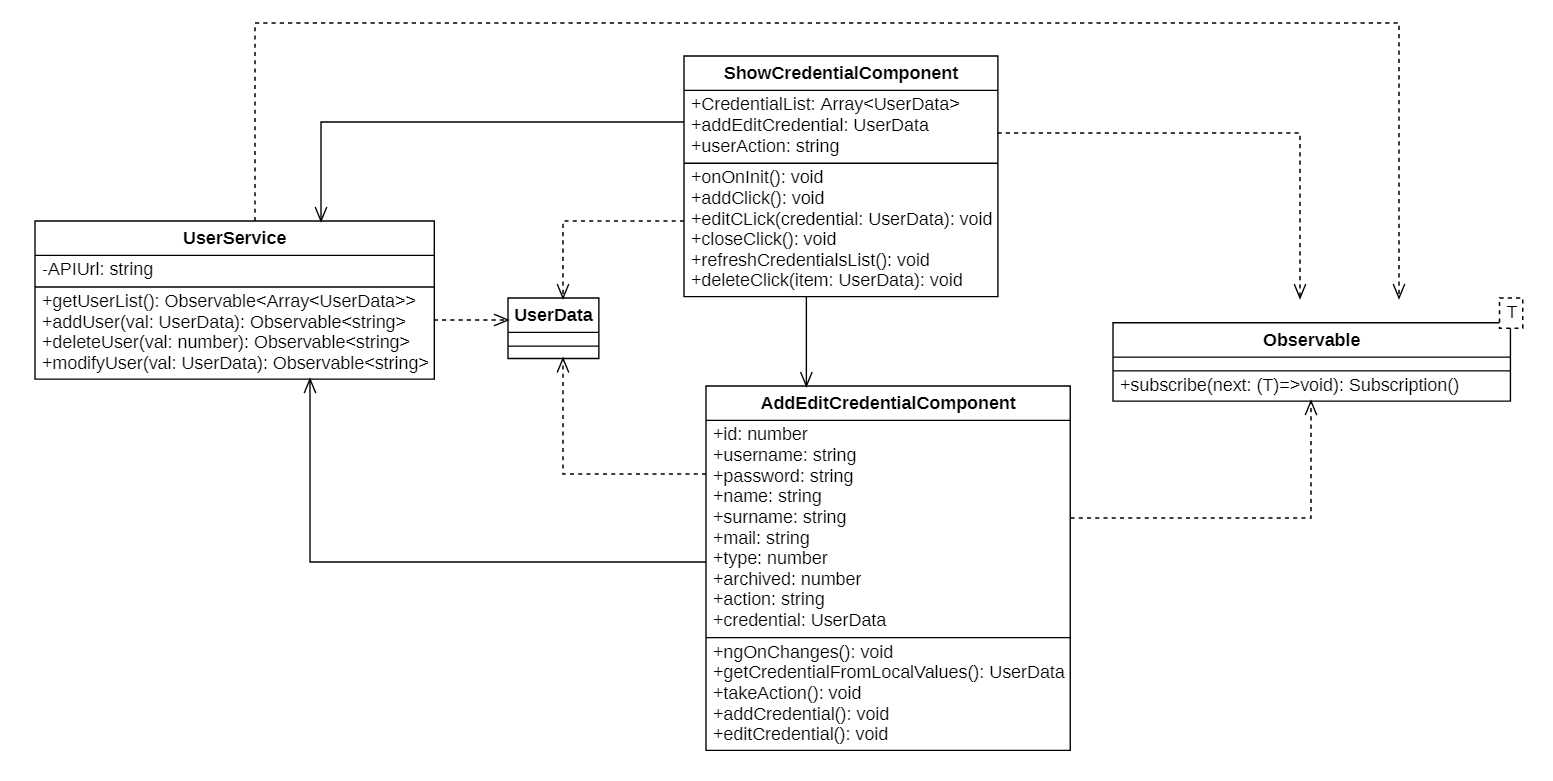
\includegraphics[width=18cm]{res/images/webapp-credenziali-diagrammaClassi.png}
	\caption{Diagramma delle classi per la gestione delle credenziali}
	\label{fig:DiagrammaClassiCredenziali}
\end{figure}
Il diagramma delle classi sovrastante rappresenta le classi coinvolte nella nella pagina di gestione delle credenziali, e le loro relazioni. Il funzionamento di questa pagina è simile a quello della pagina di gestione delle stanze e delle postazioni (§3.6.2). Qui la classe \texttt{ShowCredentialComponent} si occupa di ottenere la lista delle credenziali dal servizio \texttt{UserService} tramite oggetti \texttt{Observable}. Essa delega alla classe \texttt{AddEditCredentialComponent} l'aggiunta e modifica di credenziali. Il passaggio delle informazioni riguanti le credenziali viene sempre attuato tramile oggetti della classe \texttt{UserData}.

\paragraph{Classi}
\subparagraph{ShowCredentialComponent}
Classe che si occupa della visualizzazione di una lista delle credenziali ottenute tramite il service \texttt{UserService}. \newline
\textbf{Attributi}
\begin{itemize}
	\item \texttt{+ CredentialList: Array<UserData>} \newline
	Array nel quale vengono salvate le credenziali ottenute dal service.
	\item \texttt{+ addEditCredential: UserData} \newline
	Variabile utilizzata per il passaggio delle informazione da questa classe a \texttt{AddEditCredentialComponent}. Il valore di questa variabile viene assegnato alla variabile \texttt{credential} di quest'ultima classe.
	\item \texttt{+ userAction: string} \newline
	Variabile utilizzata per la selezione del tipo di azione (aggiunta o modifica) da eseguire. Il valore di questa variabile viene assegnato alla variabile \texttt{action} di \texttt{AddEditCredentialComponent}.
\end{itemize}
\textbf{Metodi}
\begin{itemize}
	\item \texttt{+ ngOnInit(): void} \newline
	Metodo chiamato all'inizializzazione della pagina. Provoca l'aggiornamento della lista di credenziali.
	\item \texttt{+ addClick(): void} \newline
	Metodo chiamato nel momento in cui l'utente apre il form di creazione di una credenziale. Imposta \texttt{userAction} e \texttt{addEditCredential} in modo che possano essere usate per aggiungere una credenziale as sistema.
	\item \texttt{+ editClick(credential: UserData): void} \newline
	Metodo chiamato nel momento in cui l'utente apre il form di modifica di una credenziale. Imposta \texttt{userAction} e \texttt{addEditCredential} in modo che possano essere usate per modificare la credenziale.
	\item \texttt{+ closeClick(): void} \newline
	Metodo chiamato nel momento in cui l'utente chiude il form di creazione di una credenziale. Provoca l'aggiornamento della lista di credenziali.
	\item \texttt{+ refreshCredentialsList(): void} \newline
	Provoca l'aggiornamento della lista di credenziali tramite \texttt{UserService}.
	\item \texttt{+ deleteClick(item: UserData): void} \newline
	Metodo chiamato nel momento in cui l'utente preme sul pulsante per l'eliminazione di una credenziale. Provoca l'eliminazione tramite \texttt{UserService}.
\end{itemize}
\subparagraph{AddEditCredentialComponent}
Classe che si occupa della creazione e modifica di credenziali da parte dell'utente. I primi 8 attributi sono modificabili dall'utente tramite un form e definiscono i valori della credenziale che si sta creando o modificando. \newline
\textbf{Attributi}
\begin{itemize}
	\item \texttt{+ id: number}
	\item \texttt{+ username: string}
	\item \texttt{+ password: string}
	\item \texttt{+ name: string}
	\item \texttt{+ surname: string}
	\item \texttt{+ mail: string}
	\item \texttt{+ type: number}
	\item \texttt{+ archived: number}
	\item \texttt{+ action: string} \newline
	Variabile che determina il tipo di azione da eseguire ( aggiunta o modifica della credenziale). Viene impostata dalla classe \texttt{ShowCredentialComponent}.
	\item \texttt{+ credential: UserData} \newline
	Variabile attraverso la quale questa classe ottiene i valori iniziali della credenziale che dovrà essere modificata o aggiunta. Viene impostata dalla classe \texttt{ShowCredentialComponent}.
\end{itemize}
\textbf{Metodi}
\begin{itemize}
	\item \texttt{+ ngOnChanges(): void} \newline
	Metodo chiamato ogni volta che uno degli attributi data-bound, in questo caso \texttt{action} e \texttt{credential} viene modificato. Viene utilizzato per aggiornare i primi 8 attributi in base al valore dell'ultimo, che viene impostato da \texttt{ShowCredentialComponent}
	\item \texttt{+ getCredentialFromLocalValues(): UserData} \newline
	Restituisce un oggetto costruito a partire dai primi 8 attributi dell classe.
	\item \texttt{+ takeAction(): void} \newline
	Avvia l'evento di aggiunta o modifica della credenziale. La scelta tra le due possibilità è determinata dall'attributo action.
	\item \texttt{+ addCredential(): void} \newline
	Aggiunge la credenziale determinata dai primi 8 valori al server.
	\item \texttt{+ editCredential(): void} \newline
	Modifica la credenziale presente sul server con id pari all'attributo \texttt{id} impostandone gli altri valori con quelli degli altri attributi.
\end{itemize}
\subparagraph{UserService}
Servizio che permette di ottenere dal server le credenziali salvate. Ogni metodo di questa classe, tranne il costruttore, restituisce un \texttt{Observable}. Questo oggetto espone un metodo subscribe con il quale si potrà impostare una funzione di callback che verrà chiamata quando il server fornirà una risposta. \newline
\textbf{Attributi}
\begin{itemize}
	\item \texttt{- APIUrl: string}
	L'url base dell'API REST a cui il servizio fa riferimento.
\end{itemize}
\textbf{Metodi}
\begin{itemize}
	\item \texttt{+ getUserList(): Observable<Array<UserData>>} \newline
	Fornisce un'array contenente tutte le credenziali presenti sul server
	\item \texttt{+ addUser(val: UserData): Observable<string>} \newline
	Permette di aggiungere una credenziale al server. Restituisce l'esito dell'operazione sotto forma di stringa.
	\item \texttt{+ deleteUser(val: number): Observable<string>} \newline
	Permette di rimuovere una credenziale dal server, specificandone l'id. Restituisce l'esito dell'operazione sotto forma di stringa.
	\item \texttt{+ modifyUser(val: UserData): Observable<string>} \newline
	Permette di modificare una credenziale presente sul server. La credenziale da modificare è specificata dall'attributo \texttt{id} del parametro \texttt{val}. I nuovi valori della credenziale sono specificati dagli altri attributi del parametro. Restituisce l'esito dell'operazione sotto forma di stringa.
\end{itemize}
\subparagraph{UserData}
Questa classe contiene tutti e soli i valori necessari per il salvataggio di un utente sul database. È utilizzata per il transito dei dati degli utenti all'interno dell'applicazione. \newline
\textbf{Attributi}
\begin{itemize}
	\item \texttt{+ id: number}
	\item \texttt{+ username: string}
	\item \texttt{+ password: string}
	\item \texttt{+ name: string}
	\item \texttt{+ surname: string}
	\item \texttt{+ mail: string}
	\item \texttt{+ type: number}
	\item \texttt{+ archived: number}
\end{itemize}
\subparagraph{Observable<T>}
Classe fornita dalla libreria Rxjs. Viene utilizzata per effettuare chiamate asincrone al server. Per una documentazione più approfondita fare riferimento a \url{https://angular.io/guide/rx-library}. \newline
\textbf{Metodi}
\begin{itemize}
	\item \texttt{+ subscribe(next: (T)=>void): Subscription} \newline
	Metodo che permette di eseguire la chiamata al server e di specificare la funzione di callback che gestirà la risposta.
\end{itemize}

\subsection{Diagrammi di sequenza}
\subsubsection{Login}
\begin{figure}[H]
	\centering
	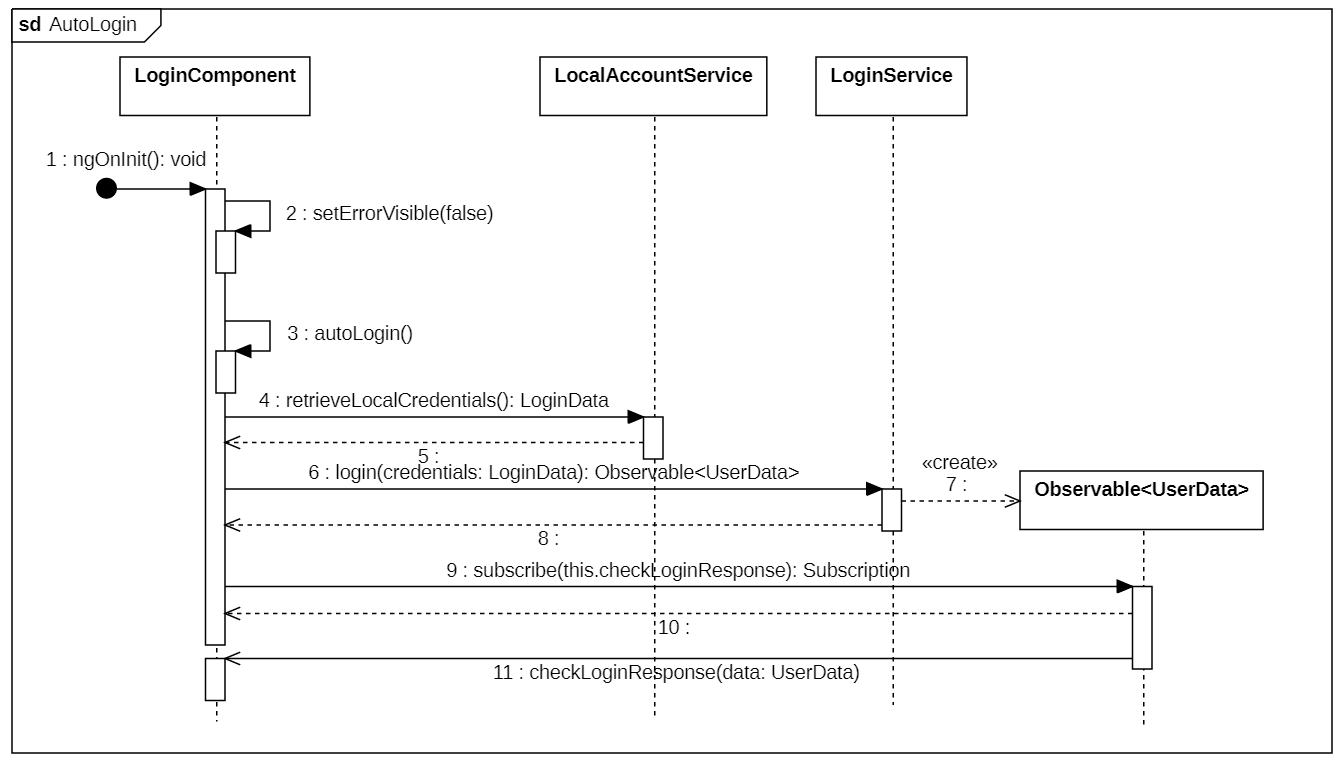
\includegraphics[width=18cm]{res/images/webapp-autologin-diagrammaSequenza.png}
	\caption{Diagramma di sequenza per l'evento di login automatico}
	\label{fig:DiagrammaSequenzaAutoLogin}
\end{figure}
Il diagramma sovrastante rappresenta l'evento di login automatico. L'evento è provocato dall'inizializzazione della pagina (\texttt{ngOnInit}). La sequenza consiste nel richiedere le credenziali salvate nel browser tramite il \texttt{LocalAccountService} ( \texttt{retrieveLocalCredentials}) e di tentare un'autenticazione al server con esse tramite il \texttt{LoginService} (\texttt{login}). In caso di esito positivo viene resituito da quest'ultimo servizio un oggetto \texttt{UserData} con i dati dell'utente che si è autenticato. La funzione \texttt{checkLogin} gestisce la risposta del server.
\subsubsection{Gestione stanze e postazioni}
\begin{figure}[H]
	\centering
	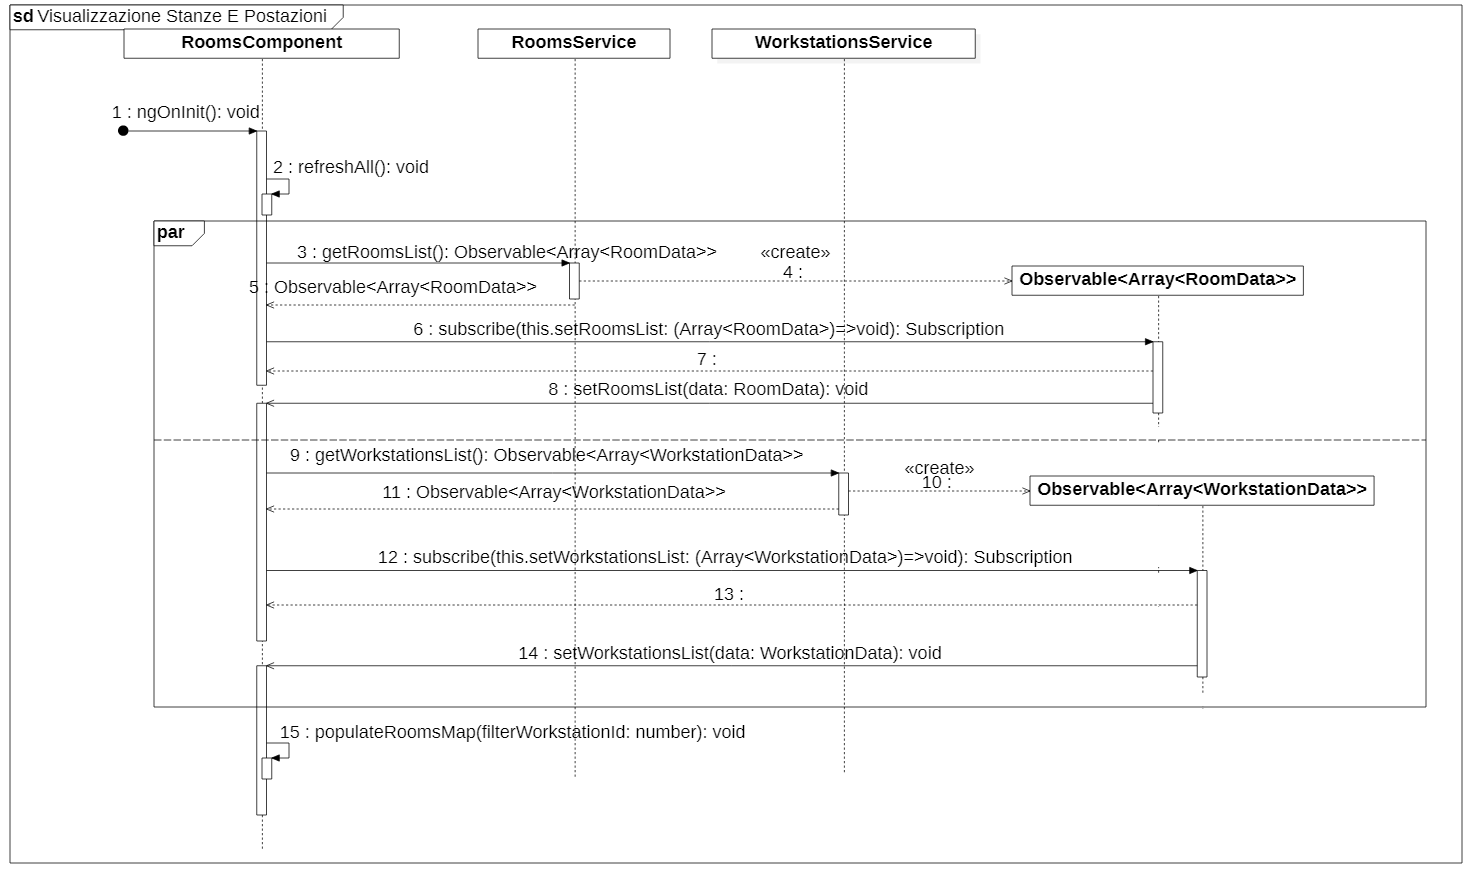
\includegraphics[width=18cm]{res/images/webapp-visualStanzePostazioni-diagrammaSequenza.png}
	\caption{Diagramma di sequenza per la visualizzazione delle stanze e delle postazioni}
	\label{fig:DiagrammaSequenzaStanzePostazioni1}
\end{figure}
Il diagramma sovrastante rappresenta un'evento scatenato dall'inizializzazione della pagina (notificata tramite la funzione \texttt{ngOnInit()}) che consiste nell'ottenimento di una lista delle postazioni e delle stanze dal server e della suddivisione delle prime in una mappa. Questa mappa verrà utilizzata dalla vista per mostrare le postazioni suddivise in stanze. L'evento rappresentato nel diagramma viene provocato ogni volta che si chiama il metodo \texttt{refreshAll()}. Questa funzionalità viene utilizzata, per esempio, dopo che una postazione è stata eliminata o modificata.
\begin{figure}[H]
	\centering
	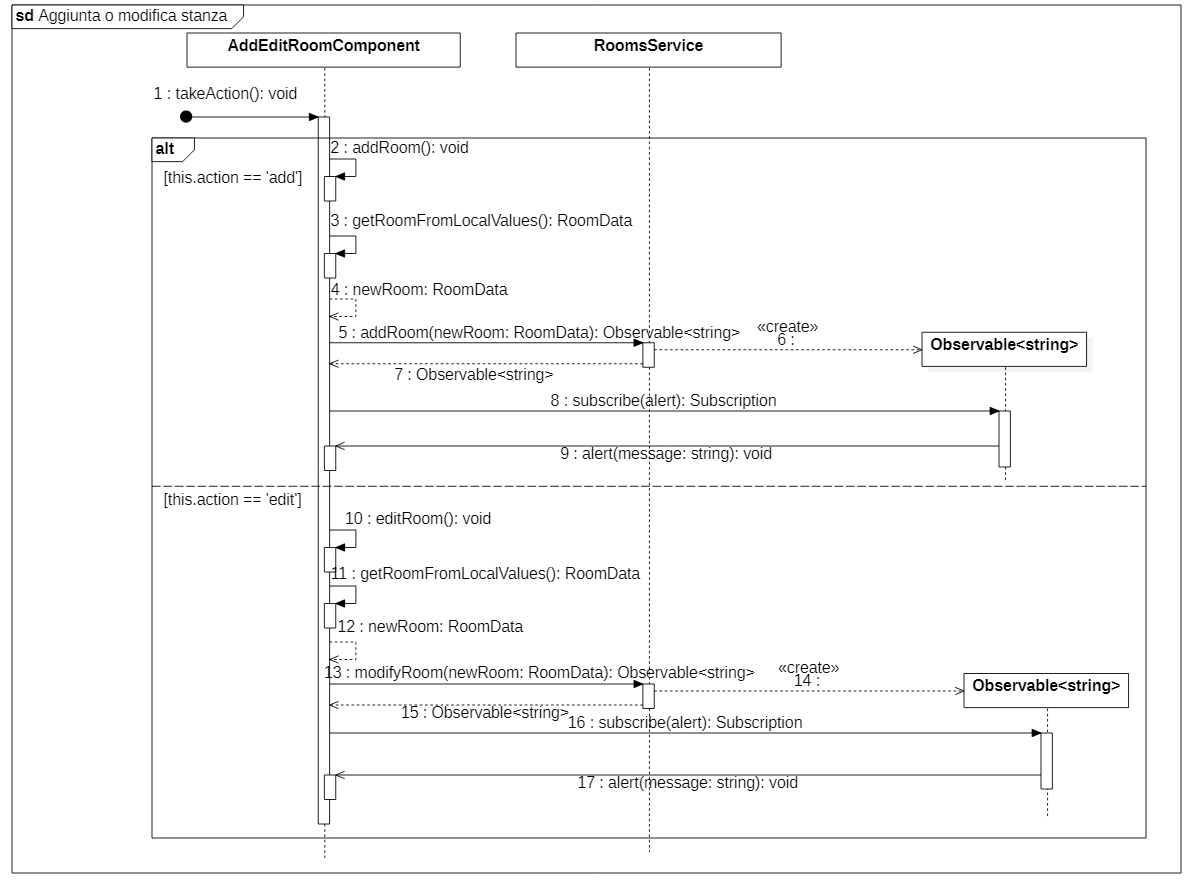
\includegraphics[width=18cm]{res/images/webapp-addEditStanzePostazioni-diagrammaSequenza.png}
	\caption{Diagramma di sequenza per l'aggiunta e la modifica di una stanza}
	\label{fig:DiagrammaSequenzaStanzePostazioni2}
\end{figure}
Il diagramma sovrastante rappresenta l'evento di aggiunta o modifica di una stanza.
In entrambi i casi l'evento è provocato dalla chiamata del metodo \texttt{takeAction()}, provocata dalla pressione di un pulsante da parte dell'utente. A questo punto la scelta dell'una o dell'altra via è determinata dal parametro \texttt{action}, che ha assunto valore 'add' o 'edit' a seconda del comportamento dell'utente.
\subsubsection{Gestione credenziali}
\begin{figure}[H]
	\centering
	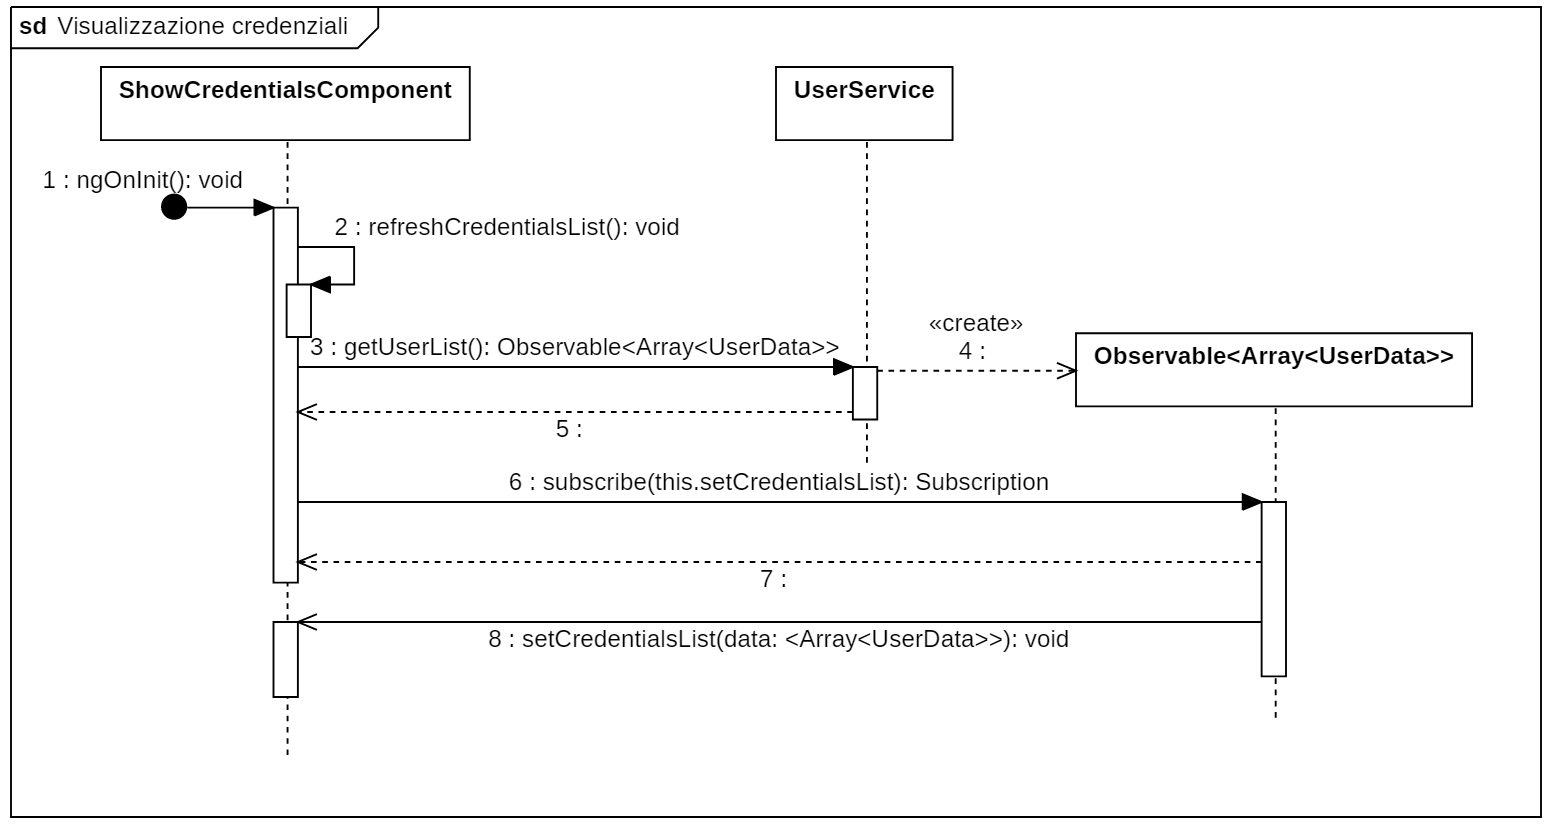
\includegraphics[width=18cm]{res/images/webapp-showCredentials-diagrammaSequenza.png}
	\caption{Diagramma di sequenza per la visualizzazione delle credenziali}
	\label{fig:DiagrammaSequenzaVisualizzazioneCredenziali}
\end{figure}
Il diagramma sovrastante rappresenta l'evento di visualizzazione delle credenziali presenti sul server. L'evento viene scatenato dall'inizializzazio della pagina (\texttt{ngOnInit}). Successivamente il componente \texttt{ShowCredentialsComponent} richiede al servizio \texttt{UserService} una lista delle credenziali. Questa lista verrà assegnata ad una variabile tramite \texttt{setCredentialsList}.
\begin{figure}[H]
	\centering
	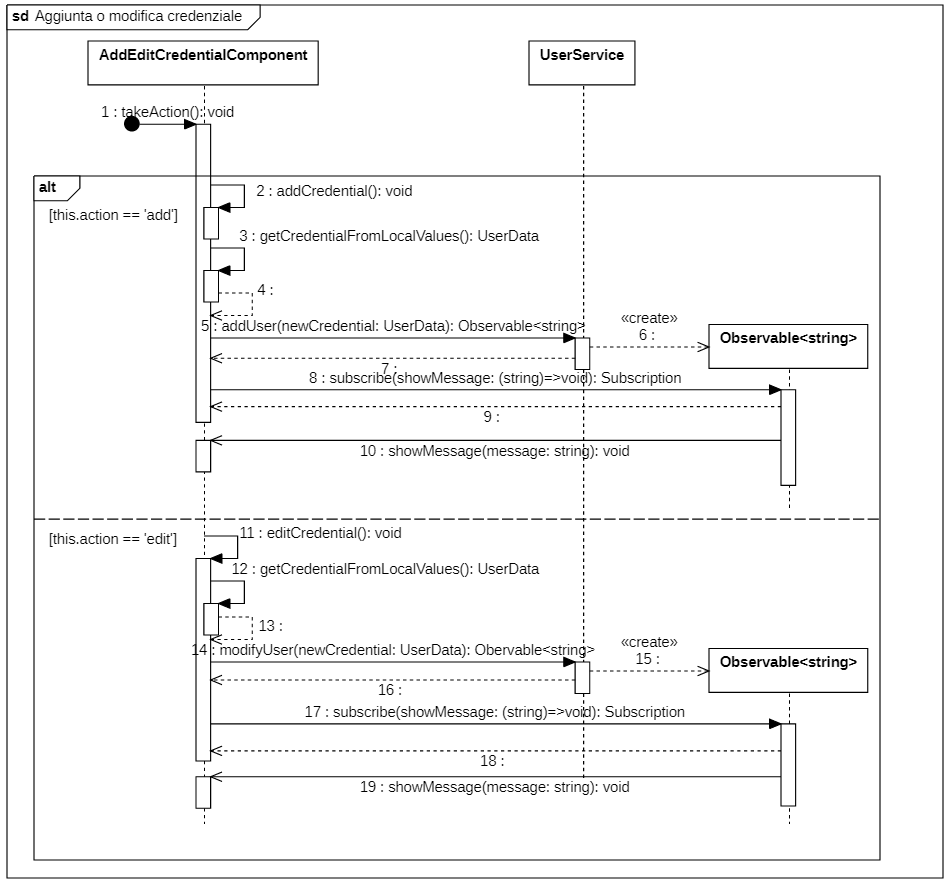
\includegraphics[width=18cm]{res/images/webapp-credenzialiAddEdit-diagrammaSequenza.png}
	\caption{Diagramma di sequenza per l'aggiunta e la modifica delle credenziali}
	\label{fig:DiagrammaSequenzaVisualizzazioneCredenziali}
\end{figure}
Il diagramma sovrastanza rappresenta l'azione di aggiunta o modifica di una credenziale da parte di un'amministratore. In entramb ii casi l'azione è provocata dalla chiamata a \texttt{takeAction}, eseguita dall'utente tramite la pressione di un pulsante. Successivamente viene eseguita l'aggiunta (\texttt{addCredential}) o la modifica (\texttt{editCredential}) della credenziale specificata dai valori inseriti dall'utente.



